\documentclass[a4paper,12pt,twoside,openright]{book}

\usepackage[a4paper]{geometry}
\usepackage[T1]    {fontenc }% Allow accented output charachters
\usepackage[utf8]  {inputenc}% Allow accented input charachters 
\usepackage        {lmodern }% Modern output font	
\usepackage		 {amsmath}%Math mode additions
\usepackage		 {amsfonts}
\usepackage{MnSymbol}
\usepackage{amsthm}
\usepackage		 {floatrow}% Append additional information to images (source)
\usepackage		{mathtools}
\usepackage[pdftex]{graphicx}% Adds the ability to include images 
\usepackage		 {xcolor   }% Colors are fun :)
\usepackage        {colortbl}% Named even more. 
\usepackage        {url     }% Makes urls clickable 
\usepackage		{array}
\usepackage		 {tikz	  }% Latex drawn figures
\usetikzlibrary{shapes,calc,positioning,decorations, trees}
\usepackage		{wrapfig}
\usepackage{fixltx2e}
\usepackage		{relsize}
\usetikzlibrary	 {matrix  }
\usepackage		{textcomp}
\usepackage        {scalefnt }% Scale the latex drawn figure elements
\usepackage[pdf]{pstricks}
\usepackage{subfigure}
\usepackage{Sweave}
\usepackage{enumerate}
\usepackage{minted}
\usepackage{titlesec}
\newcommand{\sectionbreak}{\clearpage}

% The csquotes should be used with bable to help with the references formating 
\usepackage[style=english]{csquotes} 
% Biblatex
\usepackage[style=ieee,
backend=biber,babel=other*, language=english, sorting=none,
backref=false]{biblatex} 
% Background highlight color used for the source code and the tables
\definecolor{bgSrc}{rgb}{0.95,0.95,0.95}
\colorlet{ColorGreyish}{black!10}

\usepackage[unicode]{hyperref}% - Add links between the doc
\usepackage[all]{hypcap}   %Let the links point above figures and not below
\usepackage[numbered,
			  open, 
			  openlevel=2,
			  atend]{bookmark}% - We want numbers

\usepackage{fancyhdr}
\setlength{\headheight}{20pt}

\pagestyle{fancy}
\renewcommand{\chaptermark}[1]{ \markboth{#1}{} }
\renewcommand{\sectionmark}[1]{ \markright{#1}{} }
\fancyhf{}
\fancyhead[LE,RO]{\thepage}
\fancyhead[LO]{\textit{ \nouppercase{\leftmark}} }
\fancyhead[RE]{\textit{ \nouppercase{\rightmark}} }

\fancypagestyle{plain}{ %
  \fancyhf{} % remove everything
  \renewcommand{\headrulewidth}{0pt} % remove lines as well
  \renewcommand{\footrulewidth}{0pt}
}

\usepackage{changepage,ifthen}
\newcommand\skiptooddpage{%
   \checkoddpage
   \ifthenelse{\boolean{oddpage}}%
      {\null\clearpage \null \clearpage}%
      {\null\clearpage}%
}

\usepackage{chngcntr}
\counterwithout{section}{chapter}
\counterwithout{footnote}{chapter}
\counterwithout{figure}{chapter}

\usepackage{tocbibind}

\begin{document}

% A címlap
% !TeX encoding = UTF-8 
% !TeX spellcheck =hu_HU
\hypersetup{pageanchor=false}
\begin{titlepage}
\newcommand{\HRule}{\rule{\linewidth}{0.5mm}}
\begin{center}


\includegraphics[width=0.3\textwidth]{./img/university-of-toronto-logo.png}\\
\textsc{University of Toronto}\\

% Title
\HRule \\[0.4cm]
{ \huge \bfseries Statistics: Making Sense of Data }\\[0.4cm]
{@Coursera by Alison Gibbs, Jeffrey Rosenthal} \\

\includegraphics[width=0.2\textwidth]{./img/introstatslogocropped.jpg}\\
\HRule \\[1.5cm]

% Author and supervisor
\begin{minipage}{0.4\textwidth}
\begin{flushleft} \large
\emph{Author:}\\
\textsc{Gábor} Bernát
\end{flushleft}
\end{minipage}

\vfill
% Bottom of the page
{\large \today}
\end{center}
\end{titlepage}
\hypersetup{pageanchor=false}

\tableofcontents
\chapter{Introduction}
\chapter*{Making sense of data}
\addcontentsline{toc}{chapter}{Making sense of dataset}
\setcounter{section}{0}
\renewcommand*{\theHsection}{ch1.\the\value{section}}

\section{Data categorization}

An \emph{observational unit} is the person or thing on which measurements are
taken. Note that this can also be a case, object, a subject and so on. A
\emph{variable} is a characteristic measured on the observational unit. An
instance of the variable we call the \emph{observed value} or
\emph{observation}. Variables can be of three kind:

\begin{description}
  \item[quantitive] variable take numerical values for which arithmetic
  operations make sense. The height of the people is a such variable,
  \item[caterogical] variable consist of records into which the observation
  falls into (one of several categories). For example the countries of the
  world may be classified into one of the five great continets: Europe, America,
  Africa, Asia and the Pacific,
  \item[ordinal] variable have natural order, however the difference between two
  instance of the variables does nt always make sense. A good example is grades
  given by a teacher: A, B, C, D, E, F.
   
\end{description}

\section{Quantative variables}

One way of making sense of a quantitive variable is to use the \emph{five
number summary}. Given a collection of a observations we can calculate the: 

\begin{description}
  \item[Minimum] is the lowest observation value.
  \item[Maximum] is the highest observation value.
  \item[Median] is the center observation, average point. To find it you'll need
  to sort the observations, and then take the observation in the middle
  position.
  \item[First quartile] is the observation value at the $\frac{1}{4}$rd position
  in the sorted observation array.
  \item[Third quartile] is the observation value at the $\frac{3}{4}$rd position
  in the sorted observation array.
\end{description}

A graphical representation of this five values is possible via the
\emph{boxplot} as shown on figure \ref{fig:boxplot}. On the boxplot the whiskers
show the minimum and the maximum values.

\begin{figure}[htbp]
\label{fig:boxplot}
\caption{A simple way to represent the \emph{five number summary}.}
\includegraphics{1/boxplot-boxplot}
\end{figure}

Note that the median, first or thrid quartile may result in a non--integer
position. In this case these values are calcualted by interpolating them from
the nearby observations, with the given percentage; therefore, it may happen that
these values are not part of the variable instances.

\subsection{Modified boxplots}
Outliers (known as extreme values, or unusual observations) are hard
to study on a classical boxplot, so for them we use the modified boxplot. In
this case let us first define the inter-quartile range (noted as \emph{IQR}) as
the difference between the $3$rd and the $1$st quartile. Then we can define the
inner fences as the:

\begin{description}
  \item[lower fence]  is $=1$st quartile $- ~1.5\cdot $IQR, and the  
  \item[upper fence]  is $=3$st quartile $+ ~1.5\cdot $IQR.  
\end{description}

Now the lower whisker is noted as the lower fence, while the upper fence as the
upper whisker. Observations smaller than the lower fence, or larger than the
upper fence are drawn with their own circle on the plot as shown on figure
\ref{fig:boxplot_modified}.

\begin{figure}[htbp]
\label{fig:boxplot_modified}
\caption{Modified boxplots help dealing with outliers.}
\includegraphics{1/boxplot_modified-boxplot_modified}
\end{figure}

\subsection{Mean}
Given a list of observations ($x_1, x_2, \ldots x_n$), the mean of the variable
is noted as $\bar{x}$ (or $\mu$) and is calculated as: 
\[ \mbox{Mean} = \bar{x} = 
\frac{\sum{\mbox{data values}}}{\mbox{number of data points}} =
\frac{\sum_{i=1}^{n}{x_i}}{n}.
\]

However, this definition of mean is not robust, as it's easily influenced by
outlier points. Note, that in contrast the median is robust. To alleviate this
we can introduce the conept of trimmed mean, which exclude some percentage of
the lowest and highest values from the observations, before performing the same
operation to calculate the \emph{trimmed--mean}. The input of the trimmed mean
is the percentage of outliers to remove. 

\subsection{Spread of the data}

The range of the data is the difference between the maximum and the minimum.
This is not a robust measurement. The same can be told about the IQR too. The
deviation of an observation $i$ is $x_i - \bar{x}$. A good show of the spread of
the whole data is the:

\[ \mbox{variance} = \frac{\sum_{i=1}^{n}\left(x_i - \bar{x} \right)^2}{n-1}
\]

Note that we divide by one less than the count of observation points. An
intuitive explanation for this is that the first observation does not tells us
anything about deviation. The \emph{standard deviation} (also noted as $\sigma$)
is the square root of this ($\sqrt{\mbox{variance}}$), and shows the dispersion of a set of data from
its mean.

\subsection{The shape of the data - histogram}

\begin{figure}[htbp]
\label{fig:histogram}
\caption{Histogram}
\includegraphics{1/histogram-histogram}
\end{figure}

The distribution is the pattern of values in the data, showing their frequency
of occurance relative to each other. The histogram is a good way to show this
graphically; you can see an example of this on figure \ref{fig:histogram}.

Its key part is the number of \emph{bin}s used, as observations must be
separated into mutually exclusive and exhaustive bins. \emph{Cutpoints} define
where the bins start and where they end. Each bin has its own \emph{frequency},
the number of observations in it. The largest bins define the \emph{peaks} or 
\emph{modes}. If a variable has a single peak we call it an unimodal, bimodal
for two peaks and multiple peaks above that.

\begin{figure}[htbp]
\label{fig:histogram_skewed}
\caption{Skewed histograms}
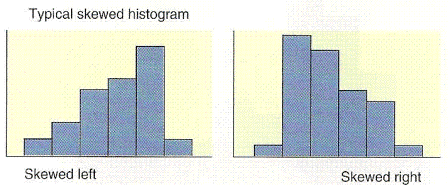
\includegraphics{img/skewed.png}
\end{figure}

Uniform distribution is a case when all the data values occur around the same
times, so we have no peaks, and such the variable has no mode. The tails of the
histogram are on its left or right side, where its extreme values are. A
histogram is left skewed if it has the left tail larger than the right, and
right skewed if the right tail  is larger than its left. 

\subsection{Empirical rule}

The empirical rule (also know as three $\sigma$ rule) states that for a normal
distribution $68\%$ of the data is within one standard deviation of the mean
value, $95\%$ is within two standard deviation, and $99.7\%$ is within three
standard deviation.

\section{Categorical variables}

Caterogical variables are not represented by numbers, so all of the earlier
statistics no longer make sense. What does make sense is the frequency of the
categories, which is graphically represented either by a barchart or a piechart.

Figure \ref{fig:category_representation} shows an example of this. In case of
barcharts we may choose to normalize the frequency, by dividing it with the
total number of observations.

\begin{figure}[htbp]
\label{fig:category_representation}
\caption{Skewed histograms}
\includegraphics{1/categorical_representation-categorical_representation}
\end{figure}
\chapter*{Releationships and data collections}
\addcontentsline{toc}{chapter}{Releationships and data collections}
\setcounter{section}{0}
\renewcommand*{\theHsection}{ch2.\the\value{section}}

\section{Relationship between quantitive and categorical variables}

Relationships are at the hearth of statistic. Let us consider an example. Let
there be the unit of observation the worlds countries. Now we define on this two
variables: a quantitive one -- the life expentancy, and a caterogical one -- in
which of the six world regions they fall into. Now we want to check for instance
if life expectancy in East Asia and Pacific tends to be larger than in the
Sub-Saharan Africe. 

One way of approach is to consider the median and mean per region, and to see
where this it's larger. However, this does not tells the whole story as the
highest in one of the regions can still be a lot higher than the lowest in
another region. Box plot is a graphical way to make the comparision.

Examining the relationship between a quantitative variable and a categorical
variable involves comparing the values of the quantitative variable among the
groups defined by the categorical variable. We need to:

\begin{enumerate}
  \item Examine the centre of the data in each group.
  \item Examine the spread of the data in each group.
  \item Examine the centre of the data in each group. 
\end{enumerate}

So create a boxplot (or summary) for each categorical observation and compare.

\subsection{In the R language}

In the R lanugage we can draw a new boxplot per category to make the
comparision. To separate categories we can use the \emph{split} function, and
finally use non-modified boxplots (\emph{range} is set to $0$) to draw them,
as seen on figure \ref{fig:boxplots}: 

\begin{minted}[numbersep=5pt]{r}
lifedata = read.table('LifeExpRegion.txt')
colnames(lifedata) = c('Country', 'LifeExp', 'Region')
attach(lifedata)
lifedata[Region=='EAP', ]
lifesplit = split(lifedata, Region)
lifeEAP = lifedata[Region=='EAP',]
lifeSSA = lifedata[Region == 'SSA', ]
boxplot(lifeEAP[,2], lifeSSA[,2], range=0, border=rainbow(2), 
        names=c('EAP', 'SSA'), main="Life Expectancies: Box Plot")
boxplot(LifeExp~Region, range=0, border=rainbow(6), 
               main='Life Expectancies: Box Plot (all 6 regions)')
\end{minted}

\begin{figure}[htbp]
\label{fig:boxplots}
\caption{Boxplots to compare quantitive and categorical variables}
\includegraphics{2/boxplots-boxplots}
\end{figure}

\section{Relationship between two categorical variables}

For instance let there be the two observations the gender of persons and their
body weight. One question we can ask is that are the same count of overweight
female as man?

\subsection{Distributions}

Distribution types are:

\begin{description}
  \item[joint distribution] of two categorical variables is the frequency or
  relative frequency of the observations considered together as a combination.
  The graphical approach is to use bar plots per combination, or aggregate these
  into a stacked bar plot.
  \item[marginal distribution] is the distribution of only one of the variables
  in a contingency table (so we take the total of the rows or of the columns in
  the table -- essentially its the distribution by only one of the variables).
  \item[marginal distribution] is the distribution of only one of the variables
  in a contingency table (so we take the total of the rows or of the columns in
  the table -- essentially its the distribution by only one of the variables).
  \item[conditional distribution] of a categorical variable is its distribution
  within a fixed value of a second variable. This distribution is normalized by
  the count of the fixed value. For graphical approach a stacked plot is used,
  by using the percentage values. Two variables in a contingency table
  indedependent if the conditional distribution of one variable is the same for
  all values of other variable.
 \end{description}

\begin{description}
  \item[Simpson's paradox] is when the conditional distributions within
  subgroups can differ from condition distributions for combined observations.
  The issue behind the paradox is that behind the two categorical variables ther
  is a third lurking variable which influences the study, like for a smoking
  study, to transform the age into age groups (if we study if the people die
  or not, having more old people in a group as observations may influence the
  result).
\end{description}
\subsection{Categorical values in R}

Categorical variables read into R are always sorted alphabetically, and
therefore any statistics about it will be displayed on that order. However,
sometimes there is a better order to this variables. In this case we can use the
\emph{factor} function and its \emph{levels} paramter to set a different order
for the categories: 

\begin{minted}[numbersep=5pt]{r}
allData <- read.table('SkeletonData.txt', header=TRUE) # dataset read 
attach(allData) # now we can use the column header names as variables
BMI = factor(BMI, levels = c('underweight', 'normal', 'overweight', 
                             'obese')) # reorder categories
\end{minted}

We can even give to the categories nicer names, as we do in the following
example for the sex categorical variable (which in the file is specified by the
values $1$ and $2$): 

\begin{minted}[numbersep=5pt]{r}
Sex = factor(Sex, levels=c('1', '2'), labels=c('Male', 'Female'))
\end{minted}

To find the number of items per category use the \emph{table} command. You can
divide tis with the number of observations to get the relative frequencies:

\begin{minted}[numbersep=5pt]{r}
relfreqBMI = table(BMI)/length(BMI)
\end{minted}

Which will result in the distribution of the data:

\begin{minted}[numbersep=5pt]{r}
BMI
underweight      normal  overweight       obese 
     0.1850      0.5625      0.2025      0.0500 
\end{minted}

We can even combine the relative and non relative values in a single table: 
\begin{minted}[numbersep=5pt]{r}
cbind(freqBMI, relfreqBMI)
\end{minted}

To get joint and the conditional distribution for two categorical variables we
need to use the \emph{CrossTable} function from the \emph{gmodels} library. 

\begin{minted}[numbersep=5pt]{r}
library(gmodels)
joint = CrossTable(BMI, Sex, prop.chisq=FALSE) 
  Cell Contents # legend for the table below
|-------------------------|
|                       N |
|           N / Row Total |
|           N / Col Total |
|         N / Table Total |
|-------------------------|
Total Observations in Table:  400  
             | Sex 
         BMI |      Male |    Female | Row Total | 
-------------|-----------|-----------|-----------|
 underweight |        46 |        28 |        74 | 
             |     0.622 |     0.378 |     0.185 | 
             |     0.164 |     0.235 |           | 
             |     0.115 |     0.070 |           | 
-------------|-----------|-----------|-----------|
      normal |       166 |        59 |       225 | 
             |     0.738 |     0.262 |     0.562 | 
             |     0.591 |     0.496 |           | 
             |     0.415 |     0.147 |           | 
-------------|-----------|-----------|-----------|
  overweight |        59 |        22 |        81 | 
             |     0.728 |     0.272 |     0.203 | 
             |     0.210 |     0.185 |           | 
             |     0.147 |     0.055 |           | 
-------------|-----------|-----------|-----------|
       obese |        10 |        10 |        20 | 
             |     0.500 |     0.500 |     0.050 | 
             |     0.036 |     0.084 |           | 
             |     0.025 |     0.025 |           | 
-------------|-----------|-----------|-----------|
Column Total |       281 |       119 |       400 | 
             |     0.703 |     0.297 |           | 
-------------|-----------|-----------|-----------|
\end{minted}

\begin{figure}[H]
\label{fig:two_categorical}
\caption{Relationship between two categorical variables}
\includegraphics[width=0.8\textwidth]{2/two_conditional-two_conditional}
\end{figure}

At this point the \texttt{joint} contains four tables: a contingency table
(frequencies -- \texttt{joint\$t}), two conditional distribution (one per point
of view -- sex \texttt{joint\$prop.col} or BMI \texttt{joint\$prop.row}), and
one displaying relative frequencies (joint distribution --
\texttt{joint\$prop.tbl}). We can use barplots to visualize this:

\begin{minted}[numbersep=5pt]{r}
layout(matrix(c(2,2,1,1), 2, 2, byrow = TRUE))
# side by side barplot
barplot(joint$t, beside=TRUE, col=rainbow(4), ylab='Frequency', 
                                              xlab='Sex')
# add legend information, 15 = plotting symbol, a little square
legend('topright', c('underweight', 'normal', 'overweight', 'obese'), 
                                            pch = 15, col=rainbow(4))
#stacked barplot
barplot(joint$prop.col, beside=FALSE, col=rainbow(4), 
                                      ylab='Frequency', xlab='Sex')
\end{minted}

as you can see it on figure \ref{fig:two_categorical}.

\section{Relationship between two quantitive variables}

One approach is to convert one (or both) of the quantitive variables into
categorical variable and then just use the already seen methods. One way to
create good groups is to use the quartile breakdown. However, this does not uses
the full information of the quantitive variables. 

One way to use it is to use a scatterplot (that is to use the quantitive
variable pairs as points in the space). On this we can use regression techniques
to fit a line on the points, effectively finding the relationship between the
variables (correlation means a rising line)

A numerical representation of this is the \emph{correlation}. Let there be two
variables indicated by the series $x_1, x_2, \ldots, x_n$ and $y_1, y_2, \ldots
y_n$, the correlation is calculated as:

\[ \mbox{correlation} = \frac{\sum_{i=1}^{n}\left( x_i-\bar{x}\right) \cdot
\left( y_i - \bar{y}\right)}{\sqrt{\sum_{i=1}^{n}\left( x_i-\bar{x}\right)^2
\cdot \sum_{i=1}^{n}\left( y_i - \bar{y}\right)^2}}
\]

Correlation values are between $[-1, 1]$, where $1$ is perfect match, and $-1$
is the perfect negative. If this is a positive value when one increases the
other tends to follow. However, note that this only captures the linear aspects
of the relationship.

\subsection{In the R lanuage}

For calculating the correlation we can use the \emph{cor} function.
 
\begin{minted}{r}
Countries = read.table('LifeGDPhiv.txt')
colnames(Countries) = c('Country', 'LifeExp', 'GDP', 'HIV')
attach(Countries)
plot(GDP, LifeExp, xlab='GDP(2000USD)', ylab='Life Expectancy (years)', 
     main='Scatterplot: Life Expectancy versus GDP per capita')
cor(GDP, LifeExp)
[1] 0.6350906
cor(LifeExp, GDP)
\end{minted}

\begin{figure}[htbp]
\label{fig:correlation}
\caption{Relationship between two quantitive variables}
\includegraphics[width=0.8\textwidth]{2/correlation-correlation}
\end{figure}

Figure \ref{fig:correlation} shows the information visually, when drawn on a
plot.

\section{Sampling}
The goal of the statistics is to make rational decision or conclusion based on
the incomplete information that we have in our data. This process is knows as
\emph{statistical inference}. The question is that if we see something in our
date (like a relationship between two variables) is it due to chance or a real
relationship? If it's not due to change then what broder conclusions we can
make, like generalize them to a larger group, or does it supports a theoretical
model? In this process the data collection has a major significance.

We collect data from the real world, however our scientific and
statistical models are part of a theoretical world. 

\begin{description}
  \item[population] the group we are interested in making conclusion about.
  \item[census] a collection of data on the entire population. This would be the
  best, however it's impractical due to time and cost effectiveness; or it's
  straight up impossible if by observing the item we would destroy it.
  Therefore, in practice we sample the population; and infer conclusions from
  the sample group.
  \item[statistic] is a value calculated from our observed data. It estimates a
  feature of the theoretical world.
  \item[paramter] is a feature of the theoretical world. Statistics are used to
  estimate their values. In order to get a good estimation our sampling needs
  to be \emph{representative}.
  \item[randomisation] is the key to select representative samples. This ensures
  that we do not over-- or under--sample any part of the population.  
\end{description}

Methods to make random sampling: 

\begin{description}
  \item[Simple Random Sampling -- SRS] Each possibly sample size of $n$ (the
  sample size) from the population is equally likely to be the sample that is
  choosen. A pratical example of this is taking out balls from a hat. 
  \item[Stratified sampling] Divide the population into non--overlapping
  subgroups called strata and choose a SRS within each subgroup. Provinces and
  states are a practical instances of stratas. This performs better when we may
  want to compare stratas, or can allow to better see traits if something is
  only characteristic to only some of the stratas (which otherwise would be
  hidden on the whole sample space).
  \item[Cluster sampling] Divide the population into non--overlapping subgroups
  called clusters, select clusters at random, and include all individual inside
  the cluster for sampling. It's good when it's easier to select groups instead
  of members; for example if we want to study students we may choose to select
  random schools and use students inside those as samples. This does requires
  that each cluster to be representative for the whole population.
\end{description}

There are also non--random sampling techniques:

\begin{description}
  \item[Systematic sampling] Select every $k$--th individual from a list of the
  population, where the position of the first person choosen is randomly
  selected from the first $k$ individuals. This will give a non--represenative
  sample if there is a structure to the list. This is fine if in the ordering of
  the population has no meaning.
  \item[Conveniance or Voluntar sampling] Use the first $n$ individuals that are
  available or the individuals who offer to participate. This is almost sure to
  give a non--representative sample which cannot be generalized to the
  population.
\end{description}

If the sample is not representative it can induce \emph{bias} into our results,
that is that it differs from its corresponding population in a systematic way.
Bias types are:

\begin{description}
  \item[Selection bias] occurs when the sample is selected in such a way that it
  systematically excludes or under--represents part of the population. For
  instance poll by using only land line phones (misses the cellular population).
  \item[Measurement or Response bias] occurs when the data are collected in such
  a way that it tend to result in observed values that are different from the
  actual value in some systematic way. In case of a poll this shows in terms of
  ill formed questions.
  \item[Nonresponse bias] occurs when responses are not obtained from all
  individuals selected for inclusion in a sample. An example of this is in a
  poll working parents tend to not respond, so their sampling will be under
  represented.
\end{description}

\section{Observational studies}

Whenever we want to compare the effect of variables on each other we need to
construct a study, for which sampling is really importat. Let us assume that we
have two (or more) groups,  and we want to compare a \emph{response variable}
(\emph{outcome}) between them. An \emph{explanatory variable} is a variable that
can be used to possibly explain the differences in the response variable between
groups (cause $\Rightarrow$ effect).

In the study we want to avoid \emph{confounding variables}, which differ between
groupsa and may effect the response variable so we can't tell what causes the
differences between groups. For instance if one were to study the effect of pot
on the IQ of the person, here a confounding variable is the social alternative
(which governs the IQ better, than the pot itself). 

Data collection methods include anecdotes (this are not representative),
observational studies and experiments. Experiments differ from observational
studie is the strength of the conclusion we can make, which is higher for the
experiment.

In observational studies we just observe existing characteristics of a subset of
individuals inside the population. The goal is to make conclusion about the
population based on the samples, or to conclude the relationship between groups
or variables in the sample. 

In this scenario the investigator has no control on which individual in which
group belongs or about any of their characteristic, as opposed to the experiment
where he can add some kind of intervention. 

The relationship between the outcome and the explanatory variable may be:

\begin{description}
  \item[causes] explanatory variable $\Rightarrow$ outcome (drinking coffe
  results in a longer life)
  \item[reverse causation] outcome $\Rightarrow$ explanatory variable (people
  with health issues avoid drinking coffe, though the longer life)
  \item[coincidence] pure chance
  \item[common cause] both of them are effected by another variable (who have
  diabiates drink less coffee, however due to their sickness have shroter life)
  \item[confounding variable] they vary with the explanatory variable. If one
  changes the other changes with it (smokers tend to drink more cofee, however
  this also effects the expected life outcome)
\end{description}

\emph{Lurking variables} are variables that are not considered in the analysis,
but may effect the natuer of relationship between the explenatory variable and
the outcome. This may be a confounding variable, or the source of the common
response , or another variable that, when considered, changes the nature of the
relationship.

\section{Experiments}

Are the golden standard. Allows for making conlusions. Again the response
variable (or also know as dependent variable -- how it depends from other
variables) is the outcome of interest, measured on each subject or entity
participating in the study (this may be quantitive or categorical). Explanatory
variable (predictor or independent variable) is a variable that we think might
help to explain the value of the response variable (can also be quantitive or
categorical).

Compared to the observation study now the researcher manipulates the explanatory
variables to see the effect of them on the outcome. Tipically a researcher has
finite time, and therefore he can study only a finit number of variable values,
and such the explanatory variable tends to be a categorical one, to which we can
also refer as a \emph{factor}. The values of the factor studied in the
experiment are its \emph{levels}.

A particular combination of values for the factors is called \emph{treatment}.
An \emph{experimental unit} is the smallest unit to which the treatment is
applied to. A treatment may not be applied to a single entity, like trying out a
new study method for a class results in a single experimental unit (a class)
instead of the count of the students inside the class.

\begin{description}
  \item[extraneous factors] are not of interest in the current study, but are
  thought to affect the reponse. They need to be controlled to avoid them
  effecting the outcome. For controlling we can: 
  \begin{itemize}
  \item Hold it constant. This limits the generilization of the study, however
  it also eliminates turning the extraneous variable into a confounding one.
  \item Use blocking, where block are groups of experimental units that are
  similar. All treatments are assigned to experimental units within each block.
  So for instance in a vaccine testing we create age groups, and each group will
  have have members getting any one of treatments, however the group as a hole,
  receives all the vaccines.
\end{itemize}
  However, this still does not solves the problem of extranous or unknown
  variables. To bypass this we need to use randomisation to assign experimental
  units to treatment groups.
\end{description}

Once we've eliminated other differences between the treatment groups, if the
response variable is different among the groups, the only explanation is the
treatment and casual conclusions can be made.

Fundamentals of experimental design:

\begin{enumerate}
  \item \emph{Control} the identified extraneous variables by blocking or
  holding them constant.
  \item \emph{Randomisation} -- is to randomly assign expermintal units
  to treatment groups.
  \item \emph{Replication} -- induce it. Not repeat the experiment, but to apply
  each treatment to more than one experimental unit. This allows to measure
  variability in the measurement of the response (which in turn also ensures
  that treatment groups are more comparable by extraneous factors, by having
  the oppurtunity of these to differ between groups).
\end{enumerate}

Experiments also have a control group. This is used to make comparisions with a
treatment of interest and either does not receives a treatment (what if the
study itself causes the change to occur) or receives the current standard
treatment. It's also refered to as the comparision group.

In conclusion we can say the randomised controlled experiments are needed to
establish casual conclusion. Another technique to reduce the potential of bias
is \emph{blinding}: 
\begin{enumerate}
  \item the experimental units are blinded, so they do not know which treatment
  they have received.
  \item the researcher is blinded if s/he does not know which treatment was
  given.
\end{enumerate}

Experimetns can be single--blinded (only one type of blinding was used) or
double--blind (if both types of blinding was used). You can also use the
\emph{placebo effect}. People often show change when participating in an
experiment wheater or not they receive a treatment. It's given to the control
group. A placebo is something that is identical to the treatment recevied by the
treatment groups, except that it contains no active ingridients.

\chapter*{Introduction to Probability}
\addcontentsline{toc}{chapter}{Introduction to Probability}
\setcounter{section}{0}
\renewcommand*{\theHsection}{ch3.\the\value{section}}

\section{The need for probability}

Up to this point we've seen and focused on how to handle data available to us.
Now it's time to see what the data in the real world corresponds in the
theoretical world. The data of the real world, that we usually end up having,
can be viewed as just a sampling of the theoretical world (which has an
infinit number of data points). Even if it really isn't any more data points in
the real world (so we have collected all the existing data points) we can still
pretend that there is and construct a theoretical model around it.

We usually try to draw inferences about our theoretical world by using the data
that we have, which represents the real world. Of course, the theoretical world
may differ from the real world and we'll be interested in studying the
relationship between two world. For instance let us consider a coin toss. In the
theoretical world we \emph{expect} to get $5$ heads out of ten tosses, yet if we
were to conduct a little experiment we may end up \emph{getting} $6$ heads out
of ten tosses.

In some cases (like tossing a bottle cap) we may not even have a theoretical
model, so the question arises that what we can conclude in this case? 

\section{Probability basics}

\begin{description}
  \item[Outcomes] are possible data that our experiment may result in. The set
  of all possible outcomes is the \emph{sample space} and it's noted as $S$.
  \item[Event] is any subset of the sample space.
  \item[Probability] -- each event has it's own probability to turn true, and
  for event $A$:
  \[
  0 \leq \mbox{P}(A) \leq 1 
  \]
  For example, the probability of some outcome is $1$, as we always end up
  having some result. The probability of the comploment event (meaning that
  event $A$ is not true) is:
 \[
  \mbox{P}(\bar{A}) = 1 - \mbox{P}(A)
 \] 
\end{description}

The term probability may have multiple interpretations: applies to a theoretical
world with a theoreticaal model where the probability for an event to occur is
P$(A)$; or we can look it as a long run, meaning that if we repeat the
experiment over and over again for a long time the occurance of event $A$ is
P$(A)$ fraction of all the events; another one is the subjective one: in my
opinion the chance that the event to occur is P$(A)$.

\section{Probability distributions}

For a coin or bear bottle fliping we use the binomial, not ass
B$(2,\frac{1}{2})$  distribution. If the exponential of the binomial is
one, we refer to it as te Bernoulli distribution: Bernoulli$(\frac{1}{2}) =
$B$(1, \frac{1}{2})$. The rolling of a dice is a discrete uniform
distribution.

\emph{Mean} is the expected value, what it equales ,,on average'' 

\[ \mbox{mean} = \mu = \sum_{x}x\mbox{P}(x)
\]

For instance in case of a rolling dice with six side:

\[
\mbox{mean} =
1\cdot\frac{1}{6}+2\cdot\frac{1}{6}+3\cdot\frac{1}{6}+4\cdot\frac{1}{6}+5\cdot\frac{1}{6}+6\cdot\frac{1}{6}=\frac{7}{2}=3.5
\]

For flipping two coins, with $Y$ being the total number of heads: 

\[
\mbox{mean}=E(Y)= 0\cdot\frac{1}{4}+1\cdot\frac{1}{2}+2\cdot\frac{1}{4} = 1
\]

\emph{Variance} in the theoretical world measures the spread of the values from
their mean value. The formula is:

\[
\mbox{variance} = \sum_{x} (x-\mu)^2\cdot\mbox{P}(x) 
\]

So for one coing flipping:

\[ \mbox{variance} =  \left(1-\frac{1}{2}\right)^2 +
\left(0-\frac{1}{2}\right)^2 + =  \frac{1}{4} \]

The \emph{standard deviation} is: 
\[ \mbox{SD} = \sqrt{\mbox{variance}} = \sqrt{\frac{1}{4}} = \frac{1}{2}
\]

The mean is linear, so any linear combination of two random variables may be
expressed with their means:

\[ \mbox{E}(aX+bY) = a\cdot\mbox{E}(X) + b\cdot\mbox{E}(Y)\]

For variance:



\begin{align*}
 \mbox{Var}(aX) &= a^2\cdot\mbox{Var}(X) \\ 
 \mbox{Var}(aX+b) &= a^2\cdot\mbox{Var}(X) \\
  \mbox{SD}(aX) &= |a|\cdot\mbox{SD}(X) 
\end{align*}

If $X$ and $Y$ are independent:
\[ \mbox{Var}(X+Y) = \mbox{Var}(X) + \mbox{Var}(Y) 
\]

Discrete random variables has a finit number of possible outcomes, and thus may
be enumerated in a form of a list. Continous random varaibles can take any value
inside an interval. An instance of this is the unifrom variable, for instance on
the interval from zero to one, meaning it's equally likeley to be any number
inside this interval. 

So for example P$(0 \leq X \leq 1) = 1$, and P$(0 \leq X \leq \frac{1}{3}) =
\frac{1}{3}$; generally speaking P$(a \leq X \leq b) = b - a$, if $0 \leq a \leq
b \leq 1$. This does mean that if $a=b$ the probability is zero, so it's easier
to think of continous probability as the area under the graph of the density
function. It's important that for any density function the total area of the
entire graph to be equal with $1$.

Uniform distributions are of a form of square function, however other functions
exist to like the exponential$(1)$ function has the form of: 

\[
 f(x) =
  \begin{cases}
   e^{-x} & \text{if } x > 0 \\
   0       & \text{if } x \leq 0
  \end{cases}
\]

The standard normal (Gaussian) distribution (bell--curve): 

\[ f(x)=\frac{1}{\sqrt{2\pi}} \cdot e ^{-\frac{x^2}{2}}\]

New bell--curves may be constructed by shifting the upper with $\mu$ (making it
the new center point) and stretching it by a factor of $\sigma$, and is noted as
Normal$(\mu, \sigma^2)$. If we have a random variable $X$ from this newly
constructed normal distribution we may transform it into a standard normal
distribution by: 

\[ 
Z = \frac{X - \mu}{\sigma} , \mbox{~ where $Z ${\raise.17ex\hbox{$\scriptstyle\mathtt{\sim}$}} Normal} (0,1). 
\]

For expected values and standard deviation now we use integals instead of sums,
for example the expected value of the uniform distribution between $0$ and $1$
is:

\[ \mbox{E}(X) = \int_{0}^{1}x\mbox{d}x = \frac{1}{2}  \]

with it's variance:

\[ \mbox{Var}(X) = \int_{0}^{1}\left(x - \frac{1}{2}\right)^2\mbox{d}x =
\frac{1}{12}
\]

For the exponential distribution it's expected value is:

\[ \mbox{E}(X) = \int_{0}^{\infty}x\cdot e^{-x}\mbox{d}x = 1  \]

with it's variance:

\[ \mbox{Var}(X) = \int_{0}^{\infty}\left(x - 1\right)^2\cdot e^{-x}\mbox{d}x =
1 \]

For the $X ${\raise.17ex\hbox{$\scriptstyle\mathtt{\sim}$}} Normal $(0,1)$: 

\[ \mbox{E}(X)  = \int_{-\infty}^{\infty}x \cdot \frac{1}{\sqrt{2\pi}}
\cdot e^{-\frac{x^2}{2}} \mbox{d}x = 0 
\]

\[ \mbox{Var}(X)  = \int_{-\infty}^{\infty} \left(x - 0\right)^2 \cdot
\frac{1}{\sqrt{2\pi}} \cdot e^{-\frac{x^2}{2}}\mbox{d}x = 1 
\]

And in case of $Y ${\raise.17ex\hbox{$\scriptstyle\mathtt{\sim}$}} Normal
$(\mu,\sigma^2)$ the mean is $\mu$, variance of $\sigma^2$ and standard
deviation of $\sigma$.

\section{Long running averages} 

What happens if you repeat an experiment lots of times and you look at the
average value you get. For example if you start flipping a coin a lot of times
and you look at the fraction of times you get head, you expect that the more you
do it, the more this comes closer to half. If you were to draw the probabilities
of the coin flip on a graph, you'd observe that the shape starts to resemble the
density function for the normal distribution. The same is the case for dice
rolling at looking the average of the rolled numbers.

\emph{The Law of Large Numbers} states that if an experiment is repeated over
and over, then the average result will converge to the experiment's expected value.

\emph{The Central Limit Theorem} states that if an experiment is repeated over
and over, then the probabilities for the average result will converge to a
Normal--distribution.

Suppose that an experiment is repeated over and over, with outcomes: $X_1, X_2,
$ $~\ldots$ and suppose each mean is E$(X_i) = m$, and each variance is is
Var$(X_i)=v$. Now let $\bar{X} = \frac{X_1 + X_2 +\ldots + X_n}{n}$ be the
average outcome. In this case we can say that:

\[ \mbox{E}(\bar{X}) = \frac{\mbox{E}(X_1) + \mbox{E}(X_2) + \ldots +
\mbox{E}(X_n)}{n} = \frac{nm}{n} = m,\]

\[ \mbox{Var}(\bar{X}) = \frac{\mbox{Var}(X_1) + \mbox{Var}(X_2) + \ldots +
\mbox{Var}(X_n)}{n} = \frac{nv}{n^2} = \frac{v}{n},\]

so we can conclude as n rises to infinity the variance (uncerteinty) becomes
smaller and smaller, tending to zero; with this the standard deviation too.

The centreal limit theorem also is responsible for the emparical rule; the
percentages are true for the graph of the normal distribution. In conclusion we
can say that all that is some kind of average, or is made up of lots and lots of
small contributions usually has a normal distribution behind it.

\section{Sampling distribution}

From the real world we collect samples, which can be considered as part of the
theoretical worlds population. We have scientific and statistical models in the
theoretical world which have parameters of features that we do not know. We use
the science of statistics to estimate them.

Let there be $p$ our parameter of interest, what we are observing, and let it
denote the number of heads of a coin flip sequence. From the real world (data)
we get some result. With this we can esitmate the parameter as:

 \[ \hat{p} = \frac{\mbox{numbers of heads observed}}{\mbox{number of coin
 flips}}\].
 
 The observed value of an estimator varies from sample of data to sample of
 data. The variability of this is called the \emph{sampling variability}. The
 probability distributions of the possible value of an estimator is its sampling
 distribution.
 
 A statistic used to estimate a paramters is \emph{unbiased} if the expected
 value of its sampling distribution is equal to the value of the parameter being
 estimated (the sampling probability is the same as the theoretical
 probability). How close the distribution of the sampling gets to the parameter
 dependes on the varince of the sampling distribution. This decreases with the
 number of samples, so the more data we have the closer we get to the
 theoretical word.
 
 Following the central limit theorem for large $n$ the sampling distribution for
 a Bernoulli event (happens or not, with probability $p$) is N$\left( p,
 \frac{p(1-p)}{n}\right)$ (sampling distribution of $\hat{p}$).
 
 If we take a normal distribution as a sample distribution with a normal
 distribution theoretical model we can calculate the expected value of the
 theoretical model as the average of the sample we have, and the standard
 deviation of the theoretical model decreases with the number of data compared
 to the standard deviation of the sampling distribution
 ($\frac{\sigma}{\sqrt{n}}$). The sampling distribution of $\bar{X}$ is N$\left(
 \mu, \frac{\sigma^2}{n}\right)$.
 
 For calculating the variance dividing with $n-1$ is important to make the
 estimator unbiased, while dividing with $n$ will result in a bias estimator.
 

\chapter*{Confidence interval}

\addcontentsline{toc}{chapter}{Confidence interval}
\setcounter{section}{0}
\renewcommand*{\theHsection}{ch4.\the\value{section}}

We observe the real world in order to understand the theoretical world; for this
we'll use the scientific and statistical models divised in the theoretical world
and use data from from the real world to estimate the paramters from the model.
We do this in hope that what conclusions we can make from our models will also
hold in the real world.


Now let us imagine the experiment of tossing a fair coin ten times. This
experiment has a binomial distribution with probability $\frac{1}{2}$, however
when amassing data from the real world we will not always get this proportion,
due to the sampling having its own distribution: for example extreme events
(like getting ten heads) are very unlikely, however getting half or close to
half of them heads is likely to happen. The question arrises where do we draw
the line, what are the values well likely to get most of the time?

Sometimes we will not have a model for our events: like in the case of flipping
a beer cap. If we were to perform a single experiment and get $m$ one side
out of $n$ events we can ask: was this a likely outcome? $m$ may be a sample of
any sample distribution (with its own parameters). For instance for the beer cap
let $n=1000$ and $m=576$. Our statistical model is binomial with a $1000$
samples, however we have no idea what's the probability of the model. 

An estimation is $\hat{p}=\frac{n}{m}=\frac{576}{1000}=0.576$. This may be a
good estimate, however it may be some other number, and so we ask what elso
could $p$ be? That is what is an interval that based on our existing experiments
the probability of getting one side of the beer cap could be? We refer to this
as the \emph{confidence interval}. 

The following methods are suppose that our data was taken in a form of simple
random sampling, and that our variables are independent; something that
statistical inference requires, otherwise we may need more complicated model.

So in conclusionwe can say that the goal of statistical inference is to draw
conclusions about a population parameter based on the data in a sample (and
statistics calculated from the data). A goal of statistical inference is to
identify a range of plausible values for a population parameter. A goal of
statistical inference is to identify a range of plausible values for a
population parameter. Inferential procedures can be used on data that are
collected from a random sample from a population.


\section{Confidence intervals with proportions}

Let us follow the example of the bottle cap. We are searching for the real $p$
with the given estiamte $\hat{p}$. The expected value of $\hat{p}$ is
$\mbox{E}(\hat{p})=p$ the variance is $\mbox{Var}(\hat{p}) =
\frac{p(1-p)}{n}=\frac{p(1-p)}{1000}$. Now according to the center limit theorem
because $p$ is the addition of lots and lots of small flips, it approximately
follows the normal distribution; that is $\hat{p} \approx
\mbox{Normal}\left(p, \frac{p(1-p)}{1000}\right)$. Now by performing a
reorganization: 

\[ \frac{\hat{p}-p}{\sqrt{p\cdot\frac{1-p}{n}}} \approx \mbox{Normal}(0,1) \]

Now for a normal distribution (and according to the empirical rule) the area
between $[-1.96, 1.96]$ covers $95\%$ of the area, so most likely our sample is
from this interval. In mathematical formula:


\[ \mbox{P} \left( \left| \frac{\hat{p}-p}{\sqrt{p\cdot\frac{1-p}{n}}} \right| >
1.96\right) = 0.05 = 5\%
\]

By writing up the reverse, and expanding we can conclude that, with
$z_{\frac{\alpha}{2}} = 1.96$:

\[ \mbox{P} \left( \underbrace{\hat{p} - \overbrace{z_{\frac{\alpha}{2}}\sqrt{p
\cdot \frac{1-p}{n}}}^{\mbox{margin of error}}}_{\mbox{lower limit}} \leq p \leq
\underbrace{\hat{p} + z_{\frac{\alpha}{2}}\sqrt{p \cdot
\frac{1-p}{n}}}_{\mbox{upper limit}} \right) = 95\%
\]
This means that we are $95\%$ confident that the value of $p$ is between is
lower and upper limit. Now the true value of $p$ is not random, however
$\hat{p}$ is as we took a random sample. Now the problem with this formula is
that while we do know $\hat{p},~p$ is unknown. One solution is to make
$\hat{p}=p$; or to make $p=\frac{1}{2}$ because that's the worst case, the
widest interval we can get.

For a given confidence interval $[a,b]$ the margin of error may be calculated
as:

\begin{align*}
a &= \hat{p} - \mbox{margin of error} \\
  b &= \hat{p} - \mbox{margin of error} \\ 
  \mbox{margin of error} &= \frac{b-a}{2}
\end{align*} 

Now modifying the area under the normal distribution that we take we can get
different confidence intervals for different probabilities. Now if you specify a
bigger confidence value, like $99\%$ you'll get a widder confidence interval.
It's up to you the trade off you are willing to accept.

Now assume you want to achive an $\alpha$ probability that you're wrong. In
this instance taken the graph of the normal distribution you want to find
$z_{\frac{\alpha}{2}}$ (y axis) such that the area remaining at each and is only
$\frac{\alpha}{2}$. In this case the area between intervals
$-z_{\frac{\alpha}{2}}$ to $z_{\frac{\alpha}{2}}$ is $1-\alpha$, which we are
looking over, as now we're missing $\alpha$ of the full area.

\section{Sample size for estimating a proportion}

Now in order to get a proportion the size of the sample has a major impact.
Let's see how we can determinate the sample size we need to find a given
proportion. We do not want to go overboard with this as we may just waste
resources or induce unrequired effort to collect it. We assume that data was
collected with simple random sampling from a population.

So a margin of error is: 

\[ \mbox{margin of error} = z_{\frac{\alpha}{2}}\sqrt{p \cdot
\frac{1-p}{n}}\]

For isntance, if our confidence interval is $95\%$, then 
$\frac{\alpha}{2}=\frac{1-0.95}{2}=0.025$, and we want a margin of error of
$\beta=0.03$. The question is what $n$ should be? For $95\%$ our normal quantile
is $1.96$. So:

\[ 0.03 = 1.96\sqrt{p \cdot
\frac{1-p}{n}}\]
 
 But we do not know what $p$ will be. To bypass this we plan for the worst case
 scenario, the expression $p\cdot(1-p)$ has its maximum at $p=\frac{1}{2}$,
 which also give our maximal margin of error for a given $n$. Now we resolve the
 equation:
 
 \[ n=\left( \frac{1.96 \cdot \frac{1}{2}}{0.03} \right)^2 = 1067 \]

Confidence intervals are about our confidence in the procedure to give us
correct results -- $95\%$ confidence intervals should contain the population
parameter $p 95\%$ of the time. If simple random samples are repeatedly taken
from the population, due to the randomness of the sampling process the observed
proportion of $\hat{p}$ will change from sample to sample and so will the
confidence interval constructed around $\hat{p}$. Of these confidence intervals,
$95\%$ will include the true population proportion $p$.

Note that $p$ is a population parameter and is therefore not a random variable.
For any interval, $p$ is either contained in the interval or not. Different
margin of error will result in different number of events required, however the
sample size increases quadratically as the margin of error decreases linearly.

\section{Confidence intervals for means}

In this case the data is not a categorical one, is instead a continous variable.
In this case the expected value is $\mu = \bar{X}$, and this is also our
estimation. The variance is equal to $\frac{\sigma^2}{n}$. Again if the data is
made up of the sum of bunch of small measurements, we can assume according
to the center limit theorem that $\bar{X} \approx \mbox{Normal}\left(\mu,
\frac{\sigma^2}{n}\right).$ Again we reduce this to the standard normal
distribution to get:

\[ \frac{\bar{X}-\mu}{\sqrt{\frac{\sigma^2}{n}}}  \approx \mbox{Normal}
\left( 0, 1\right)
\]

Now the problem now is that we do not know the value of $\sigma$. What would be
a good estimation for this? One solution is to use the standard deviation of $X$
(calculated with dividing with $n-1$), noted as $s$. However, while
$\mbox{E}(s^2)=\sigma^2$, substituting this into upper formula does not gives a
normal distribution; instead we'll have a $t$ distribution with $n-1$ degrees of
freedom:


\[ \frac{\bar{X}-\mu}{\sqrt{\frac{s^2}{n}}}  \approx t_{n-1}
\]

The $t$ distribution is similar to the normal one, however not quite there.
Increasing the degree of freedom reduces the difference between these two.
With this the $z_{\frac{\alpha}{2}}$ changes also, so you'll need to use a table
to get the correct number for a given number of freedom (which is $n-1$, where $n$ is
the sample size). The marginal error may be calculated as:

\[ \mbox{marginal error}= z_{\frac{\alpha}{2}} \cdot \sqrt{\frac{s^2}{n}} \]

We can use this to calculate the true mean from a sample mean. That is with a
given confidence we can say that our true mean is somewhere inside the
calculated confidence interval, which depends from the sample mean with the
calculated marginal error.

\section{Robustness for confidence intervals}

To use these methods many conditions must be satisfied, and an important part of
the statistical inference is to determine if these hold. Here are what we need
to make sure that they are true:

\begin{enumerate}
  \item the $n$ observations are independent,
  \item $n$ needs to be large enough, so that the central limit theorem may kick
  in and $\hat{p}$ to have a normal distribution, 
\end{enumerate}

For extreme theoretical $p$ values larger counts of samples are required to
achieve the same confidence interval. For instance in case of a coin flip if $p$
is $\frac{1}{2}$ a hundred samples may be enough for the central limit theorem
to kick in and achive a $95\%$ confidence. However, if $p=0.01$ we may need
$1000$ samples for the same confidence. An explanation for this is that the
normal distribution is a continous model, and we are using it to estimate 
discrete values.

In order for the confidence interval procedure for the true proportion to
provide reliable results, the total number of subjects surveyed should be large.
If the true population proportion is close to $0.5$ a sample of $100$ may be
adequate. However, if the true population proportion is closer to $0$ or $1$ a
larger sample is required.

Increasing the sample size will not eliminate non-response bias. In the presence
of non-response bias, the confidence interval may not cover the true population
parameter at the specified level of confidence, regardless of the sample size.
An assumption for the construction of confidence intervals is that respondents
are selected independently.

In case of means the conditions are:

\begin{enumerate}
  \item the $n$ observations are independent
  \item $n$ needs to be large enough so that $\bar{X}$ is approximatly normally
  distributed.
\end{enumerate}

The $t$ distribution works extremly well with even a low number of samples ($n
=10$) if the theoretical model is a normal or skewed normal one. For this to not
be true we need some really extreme distribution, like most of the time on one
end, but has some chance for an outlier value. However, in these cases by just
increasing the mean with a constant multiplier (like to $40$) may already result
in a $90\%$ confidence value. 

Nevertheless, we also need to consider if estimating the mean is a meaningful
thing to do. Remeber that the mean is not a robust measurement, because it's
effected by outliers, something that is true for the distribution too.

A method for constructing a confidence interval is robust if the resulting
confidence intervals include the theoretical paramter approximately the
percentage of time claimed by the confidence level, even if the necessary
condition for the confidence interval isn't satisfied.

\end{document}